%%%%%%%%%%%%%%%%%%%%%%%%%%%%%%%%%%%%%%%%%
% Stylish Article
% LaTeX Template
% Version 1.0 (31/1/13)
%
% This template has been downloaded from:
% http://www.LaTeXTemplates.com
%
% Original author:
% Mathias Legrand (legrand.mathias@gmail.com)
%
% License:
% CC BY-NC-SA 3.0 (http://creativecommons.org/licenses/by-nc-sa/3.0/)
%
%%%%%%%%%%%%%%%%%%%%%%%%%%%%%%%%%%%%%%%%%

%----------------------------------------------------------------------------------------
%	PACKAGES AND OTHER DOCUMENT CONFIGURATIONS
%----------------------------------------------------------------------------------------

\documentclass[fleqn,10pt]{SelfArx} % Document font size and equations flushed left

\setlength{\columnsep}{0.55cm} % Distance between the two columns of text
\setlength{\fboxrule}{0.75pt} % Width of the border around the abstract

\definecolor{color1}{RGB}{0,0,90} % Color of the article title and sections
\definecolor{color2}{RGB}{0,20,20} % Color of the boxes behind the abstract and headings

\newlength{\tocsep} 
\setlength\tocsep{1.5pc} % Sets the indentation of the sections in the table of contents
\setcounter{tocdepth}{3} % Show only three levels in the table of contents section: sections, subsections and subsubsections

\usepackage{cite}
\usepackage{pgfgantt}
\usepackage{hyperref}
\usepackage{lipsum} % Required to insert dummy text
\graphicspath{{Figures/}}

%----------------------------------------------------------------------------------------
%	ARTICLE INFORMATION
%----------------------------------------------------------------------------------------

\JournalInfo{Plan de Trabajo de Laboratorio 6 (1er cuat. 2014)} 
\Archive{Laboratorio de Turbulencia Geof\'\i sica, DF FCEyN, UBA} 

\PaperTitle{Article Title} % Article title

\Authors{estudiante(s)\textsuperscript{1}*, Director: Dr. Pablo J. Cobelli\textsuperscript{2}} % Authors
\affiliation{\textsuperscript{1}\textit{Afiliacion estudiante(s)}} % Author affiliation
\affiliation{\textsuperscript{2}\textit{Departamento de F\'\i sica, FCEN UBA \&
IFIBA CONICET}} % Author affiliation
\affiliation{*\textbf{E-mail}: cobelli@df.uba.ar} % Corresponding author

\Keywords{Keyword1 --- Keyword2 --- Keyword3} % Keywords - if you don't want any simply remove all the text between the curly brackets
\newcommand{\keywordname}{Keywords} % Defines the keywords heading name

%----------------------------------------------------------------------------------------
%	ABSTRACT
%----------------------------------------------------------------------------------------

\Abstract{\lipsum[1]~}

%----------------------------------------------------------------------------------------

\begin{document}

\flushbottom % Makes all text pages the same height

\maketitle % Print the title and abstract box

\tableofcontents % Print the contents section

\thispagestyle{empty} % Removes page numbering from the first page

%----------------------------------------------------------------------------------------
%	ARTICLE CONTENTS
%----------------------------------------------------------------------------------------

\section*{Introduction} % The \section*{} command stops section numbering

\addcontentsline{toc}{section}{\hspace*{-\tocsep}Introduction} % Adds this section to the table of contents with negative horizontal space equal to the indent for the numbered sections

\lipsum[1-3] % Dummy text

%------------------------------------------------

\section{Motivaci\'on}

\begin{figure*}[ht]\centering % Using \begin{figure*} makes the figure take up the entire width of the page
% \includegraphics[width=\linewidth]{view}
\caption{Wide Picture}
\label{fig:view}
\end{figure*}

\lipsum[4] % Dummy text

\begin{equation}
\cos^3 \theta =\frac{1}{4}\cos\theta+\frac{3}{4}\cos 3\theta
\label{eq:refname2}
\end{equation}

\lipsum[5] % Dummy text

\begin{enumerate}[noitemsep] % [noitemsep] removes whitespace between the items for a compact look
\item First item in a list
\item Second item in a list
\item Third item in a list
\end{enumerate}

\subsection{Subsection}

\lipsum[6] % Dummy text

\paragraph{Paragraph} \lipsum[7] % Dummy text
\paragraph{Paragraph} \lipsum[8] % Dummy text

\subsection{Subsection}

\lipsum[9] % Dummy text

\begin{figure}[ht]\centering
% \includegraphics[width=\linewidth]{results}
\caption{In-text Picture}
\label{fig:results}
\end{figure}

Reference to Figure \ref{fig:results}.

%------------------------------------------------

\section{Objetivos}

\indent En esta secci\'on se describen los objetivos (tanto general como espec\'\i ficos) que se busca alcanzar en el marco del presente proyecto. 

\subsection{Objetivo general}

\indent El principal objetivo general que se persigue con el presente plan de trabajo es ...

\subsection{Objetivos espec\'\i ficos y metodolog\'\i a}

\indent Para la consecuci\'on del objetivo general descrito en la secci\'on precedente, se propone:

\section{Factibilidad del plan propuesto}

\subsection{Disponibilidad de equipamiento e insumos}

\subsection{Recursos computacionales}

\section{Cronograma de actividades}

El cronograma de las actividades a llevar a cabo, junto con su extensi\'on temporal se consigna en el diagrama de Gantt de la Fig.~\ref{fig:gantt}, para el per\'\i odo correspondiente a la cursada de Laboratorio 6 (entre la \'ultima semana de marzo y la primera de agosto). 

\begin{figure*}[ht!]
\centering
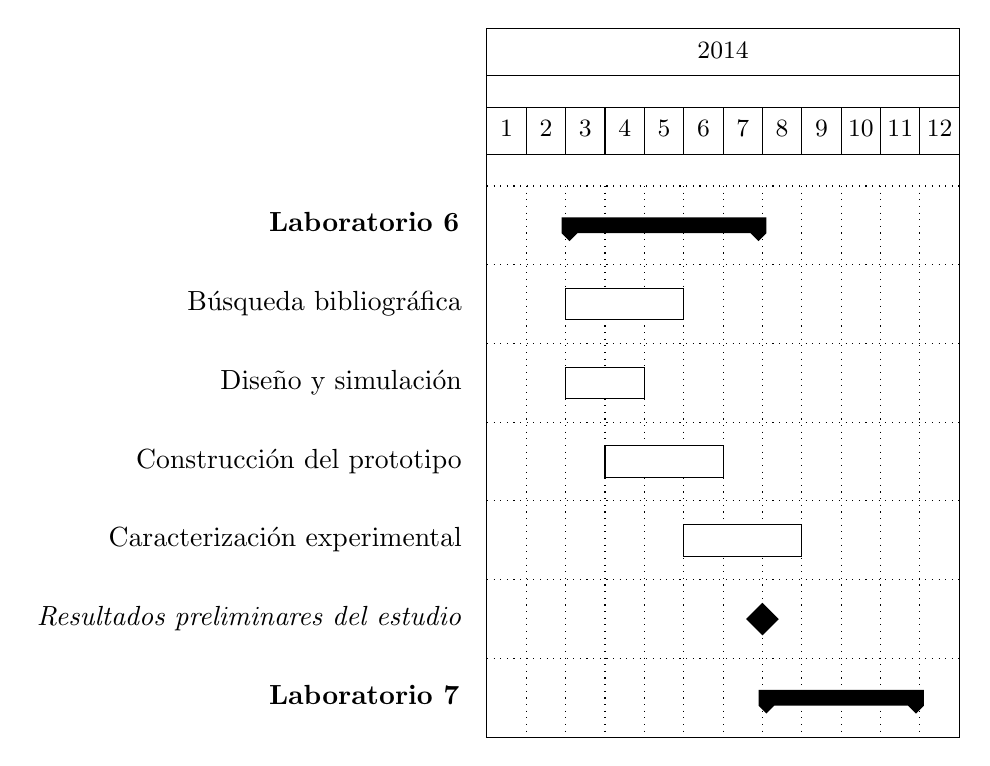
\begin{tikzpicture}
\begin{ganttchart}[vgrid={dotted}, hgrid={dotted}]{1}{12} 
\gantttitle{2014}{12} \\ 
\gantttitlelist{1,...,12}{1} \\ 
\ganttgroup{Laboratorio 6 \:}{3.75}{7} \\ 
\ganttbar{B\'usqueda bibliogr\'afica \:}{3.75}{5.5} \\ 
\ganttbar{Dise\~no y simulaci\'on \:}{3.75}{4.25} \\
\ganttbar{Construcci\'on del prototipo \:}{4.5}{6.5} \\
\ganttbar{Caracterizaci\'on experimental \:}{6.5}{8} \\
%\ganttlinkedbar{Montaje del setup experimental}{4}{6} 
% \ganttbar{Mediciones y an\'alisis preliminar \:}{6}{7} \\
\ganttmilestone{Resultados preliminares del estudio \:}{7} \\
\ganttgroup{Laboratorio 7 \:}{8}{11} 
\end{ganttchart}
\end{tikzpicture}
\caption{Diagrama de Gantt para las actividades propuestas por el presente plan de trabajo.}
\label{fig:gantt}
\end{figure*}


\section{Otra seccion}

\lipsum[10] % Dummy text

\subsection{Subsection}

\lipsum[11] % Dummy text

\begin{table}[hbt]
\caption{Table of Grades}
\centering
\begin{tabular}{llr}
\toprule
\multicolumn{2}{c}{Name} \\
\cmidrule(r){1-2}
First name & Last Name & Grade \\
\midrule
John & Doe & $7.5$ \\
Richard & Miles & $2$ \\
\bottomrule
\end{tabular}
\label{tab:label}
\end{table}

\subsubsection{Subsubsection}

\lipsum[12] % Dummy text

\begin{description}
\item[Word] Definition
\item[Concept] Explanation
\item[Idea] Text
\end{description}

\subsubsection{Subsubsection}

\lipsum[13] % Dummy text

\begin{itemize}[noitemsep] % [noitemsep] removes whitespace between the items for a compact look
\item First item in a list
\item Second item in a list
\item Third item in a list
\end{itemize}

\subsubsection{Subsubsection}

\lipsum[14] % Dummy text

\subsection{Subsection}

\lipsum[15-23] % Dummy text

%------------------------------------------------

% \section*{Acknowledgments} % The \section*{} command stops section numbering

% \addcontentsline{toc}{section}{\hspace*{-\tocsep}Acknowledgments} % Adds this section to the table of contents with negative horizontal space equal to the indent for the numbered sections

% So long and thanks for all the fish \cite{Figueredo:2009dg}.

%----------------------------------------------------------------------------------------
%	REFERENCE LIST
%----------------------------------------------------------------------------------------

\bibliographystyle{unsrt}
\bibliography{Bibliography}

%----------------------------------------------------------------------------------------

\end{document}
